%\chapter{det-comp}


%%%%%%%%%%%%%%%%%%%%%%%%%%%%%%%%%%%%%%%%%%%%%%
%\section{Anode Plane Assemblies}

%%%%%%%%%%%%%%%%%%%%%%%%%%%%%%%%%%%%%%%%%%%%%%
\section{Cathode Plane Assemblies}


\subsection{Scope, Requirements and Design Parameters}
\begin{itemize}
\item Voltage
\item Field requirements
\item FV requirements
\item Field Uniformity
\item Field cage support
\item Discharge requirements

\end{itemize}

\subsection{The need for highly resistive cathode planes}
Stored energy, charge injection to FEE, dominant ionization current density


\subsection{The design of the CPA modules}

\subsubsection{Resistive material}
%% from F. Pietropaolo

The main criteria for the selection of the resistive material to be used for the CPA panels include: 
\begin{itemize}	
\item Surface resistivity range.
\item Compatibility with cryogenic temperatures
\item Robustness to HV discharges, material ageing.
\item Radio-purity.
\item Availability on large area; achievable planarity 
\end{itemize}

Several options have been evaluated.
\begin{itemize}	
\item NORPLEX, Micarta, NP 315, phenolic laminate loaded with graphite: Intrinsic bulk resistivity in the required range (few M$\Omega$/cm). Density comparable to LAr.
\item Screen printed resistive ink on G10/FR4 substrate (~100 k$\Omega$/square) printed with specific patterns to obtain required average surface resistivity
\item DuPont resistive Kapton film  (25 $\mu$m thickness, graphite loaded, available with resistivity in the 0.5 to 50 M$\Omega$/square range) laminated on G10/FR4 substrate.
\end{itemize}
Also considered at earlier stage:
\begin{itemize}	
\item Zelec ESD powder mixed with polyurethane binder.
\item ESD surface conducting G10 from Current Composite.
\end{itemize}

Radiological tests performed at the LNGS low counting rate facility that G10/FR4 are preferable since MiCarta is more active by orders of magnitude for most relevant radioactive chains.
 
Screen printed ink and Kapton lamination on G10/FR4 are well established fabrication techniques available on panels as large as to 2.1x 1.2 m$^2$ (well matching the CPA panel required size). The screen print technique allows to choose precisely the average surface resistivity value, while Kapton exhibits a more uniform surface and resistivity. 

Tests on large size panels have demonstrated that both options survive without deformation or delamination to repeated immersions in LAr. The resistivity increase at LAr temperature is bounded to less than a factor two for both cases. Electrical contacts are performed with  specific  silver paint paste  highly stable at LAr temperature and resistant to mechanical scratches.

Tests on surface ageing when exposed to HV sparks indicate that Kapton is the preferred solution because:
\begin{itemize}	
\item in the resistive ink case, sparks tend to develop along direction of less resistivity, perpendicular to strip direction inducing a visible degradation of the material surface with some consistent ink evaporation and local measurable change in resistivity (Figure~\ref{fig:cpa-resink}).
\item in the Kapton case instead, sparks are point-like inducing tiny localized carbonization on material surface, at the spark position, but no change in average resistivity is recorded (Figure~\ref{fig:cpa-kapton}). 
\end{itemize}

\begin{cdrfigure}[Resistive ink ageing from sparks]{cpa-resink}{Resistive ink ageing from sparks. 
 {\bf Left:} spark propagation along preferred directions (lower resistivity), {\bf Right:} Status after test: degradation with some material evaporation.} 
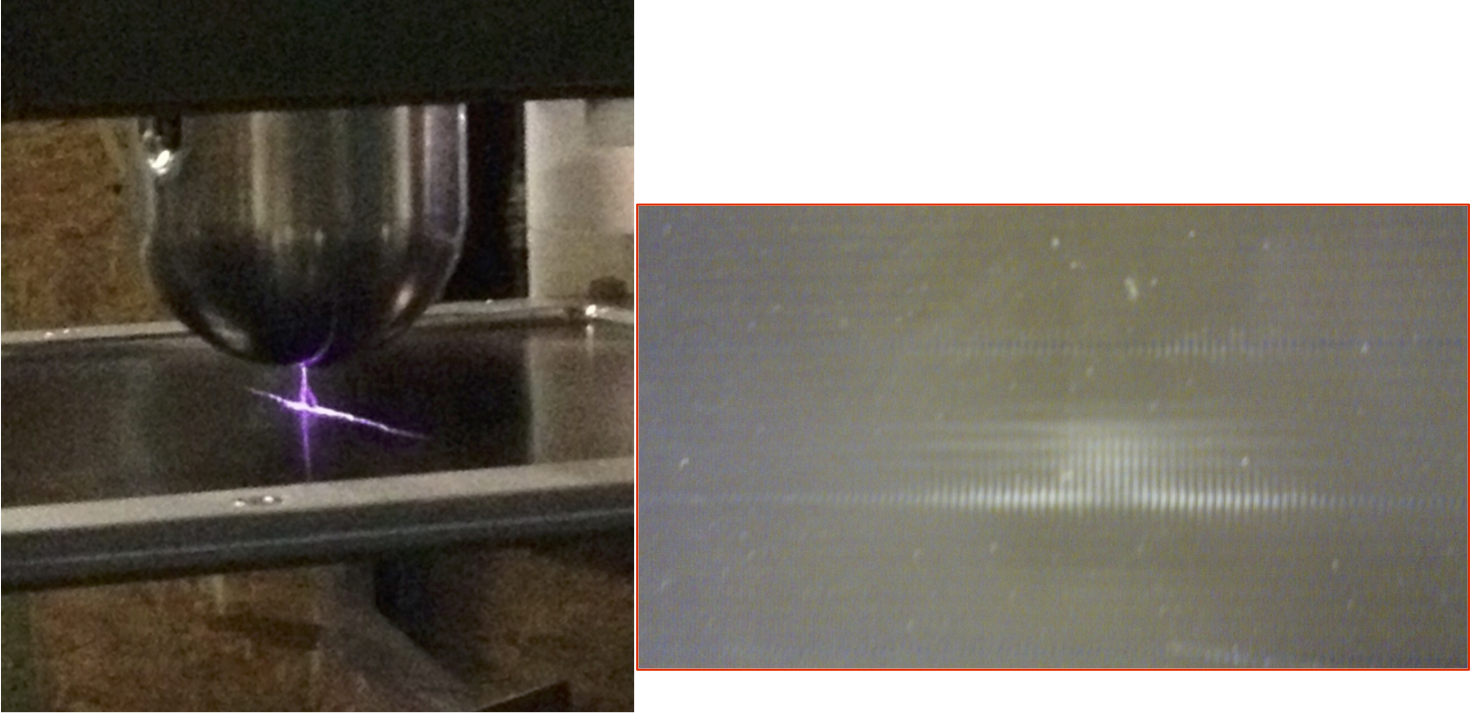
\includegraphics[width=\linewidth]{tpc_cpa-resink.png}
\end{cdrfigure}

\begin{cdrfigure}[The field cage test setup]{cpa-kapton}{Resistive kapton ageing from sparks. 
 {\bf Left:} point-like sparks. {\bf Right:} Localized carbonization on material surface, at the spark position.}
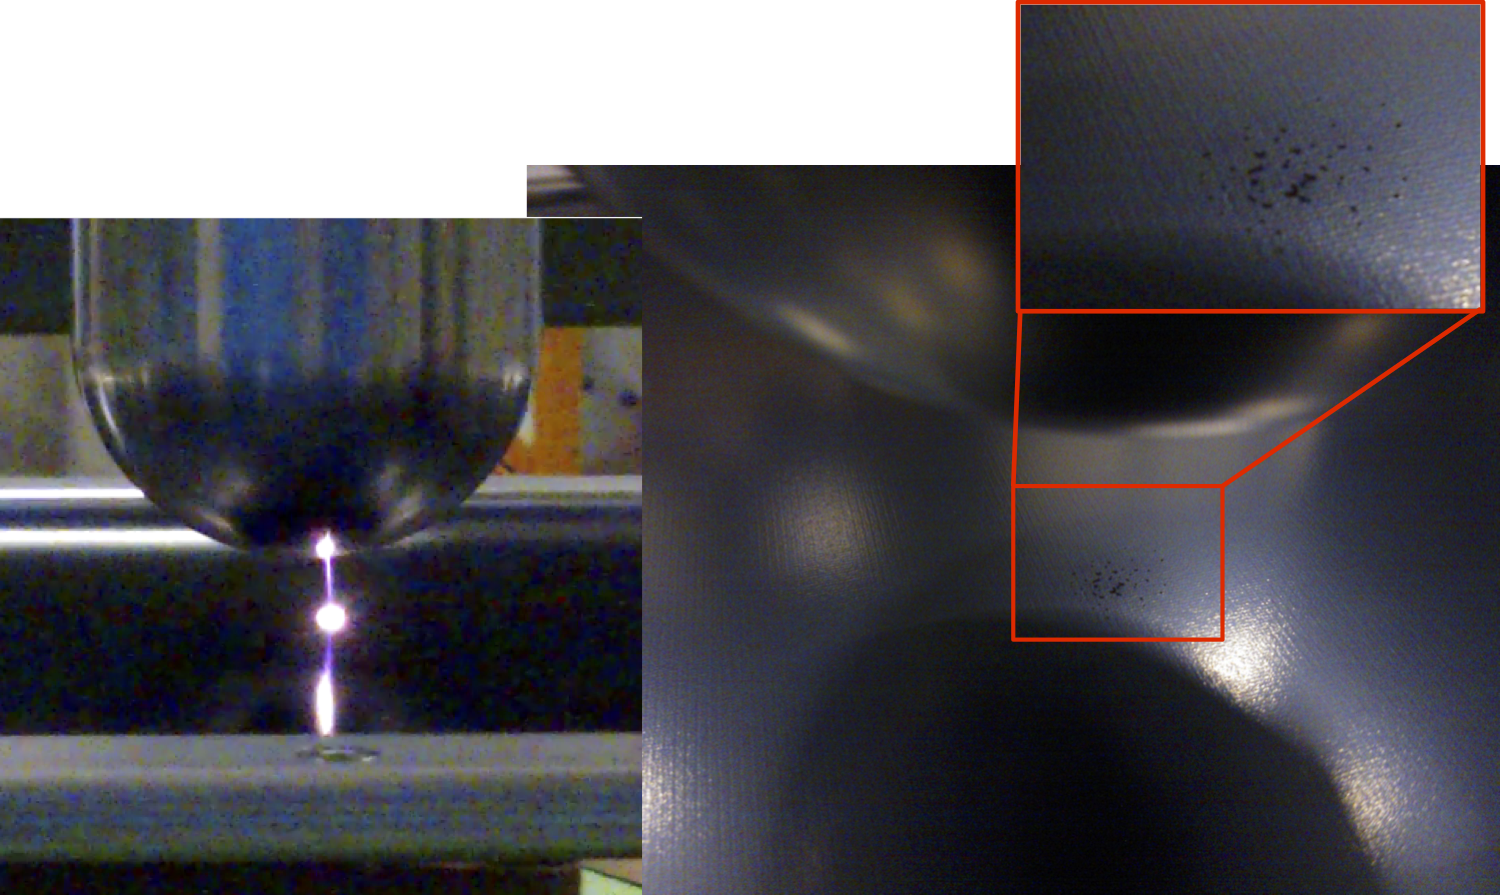
\includegraphics[width=\linewidth]{tpc_cpa-kapton.png}
\end{cdrfigure}




\subsubsection{Support frame structure}

\subsubsection{The HV distribution bus and HV feedthrough receptacle }

\subsubsection{The mechanical and electrical interconnect features between modules}

\subsection{Assembly sequence and QC procedures}

\subsection{Installation sequence}




